\chapter{Візуалізація даних.}

Людський мозок значно краще сприймає візуальні образи, ніж набори сухих чисел. За лічені секунди можна помітити тенденцію на графіку, яку не можна було б побачити в таблиці в екселі чи в базі даних. Саме тому надзвичайно важливим етапом аналізу даних є візуалізація.

Важливо підкреслити різницю між двома дуже різними поняттями, які люди описують, використовуючи загальний термін "візуалізація". Перше з них — "візуалізація для дослідження даних": використання візуалізації для розуміння (тобто для власного розуміння) сукупності даних з метою подальшого аналізу. Коротко кажучи, мета цього типу візуалізації — "знайти істину" в даних. Альтернативою є "візуалізація для презентації": виокремлення певного аспекту даних у вигляді зрозумілої діаграми або графіку, що передає широкій аудиторії конкретний аспект даних, який ви хочете донести. Цей тип візуалізації має на меті "переконати інших людей у правдивості ваших висновків".

\textit{Візуалізація VS статистика:} Візуалізація майже завжди надає більш інформативний (хоча і менш кількісний) огляд ваших даних, ніж статистика (підхід, а не галузь науки в цілому).


\section{Типи даних.}

Перед тим, як приступити до візуалізації, варто зрозуміти, з яким типом даних ви маєте справу. Це потрібно для того, щоб, у першу чергу, не помилитися із вибором методу візуалізації.

Чотири основні типи даних:

\begin{itemize}
\item \textit{Номінальні дані (Nominal data)}: категоріальні дані без внутрішнього порядку між категоріями. Наприклад, змінна "тип домашньої тварини" може складатися з класів {собака, кіт, кролик}, і між цими двома типами немає відносного порядку, це просто різні дискретні значення.

\item \textit{Порядкові дані (Ordinal data)}: категоріальні дані з внутрішньою послідовністю, але "відмінності" між категоріями не мають суто числового значення. Канонічним прикладом тут є відповіді на опитування з такими відповідями: {категорично не згоден, трохи не згоден, нейтральний, трохи згоден, категорично згоден}. Важливою особливістю тут є те, що, хоча між цими типами існує чітка послідовність, немає сенсу вважати, що різниця між "трохи згоден" і "категорично згоден" є "такою ж", як різниця між "нейтральний" і "трохи згоден".

\item \textit{Інтервальні дані (Interval data)}: числові дані, тобто дані, які можна відобразити на "числовій прямій"; важливим аспектом на відміну від порядкових даних є не "дискретна проти безперервної диференціації" (наприклад, цілочисельні значення можна вважати інтервальними даними), а той факт, що відносні відмінності в інтервальних даних мають значення. Класичним прикладом є температура (у Фаренгейті або Цельсії, що ми підкреслимо трохи пізніше): тут різниці між температурами мають значення: 10 і 15 градусів розділені такою ж величиною, як 15 і 20 (ця властивість настільки властива числовим даним, що майже дивно її підкреслювати). З іншого боку, інтервальні дані охоплюють випадки, коли нульова точка "не має реального значення"; на практиці це означає, що співвідношення між двома точками даних не має значення. Двадцять градусів за Фаренгейтом не є "вдвічі гарячішими" в будь-якому значущому сенсі, ніж 10 градусів; і, звичайно, не нескінченно гарячішими, ніж нуль градусів.

\item \textit{Дані про співвідношення (Ratio data)}: також числові дані, але співвідношення між вимірами має певне значення. Класичним прикладом тут є температура за Кельвіном. Очевидно, що, як і температура за Фаренгейтом або Цельсієм, це описує основне явище температури, але на відміну від попередніх випадків, нуль за Кельвіном має значення з точки зору молекулярної енергії в речовині (тобто її відсутність). Це означає, що співвідношення мають реальне значення: речовина при 20 градусах Кельвіна має вдвічі більше кінетичної енергії на молекулярному рівні, ніж та сама речовина при 10 градусах Кельвіна.
\end{itemize}

\ding{46} "Допустимі операції", які ми можемо виконувати над двома елементами різних типів:

Номінальні дані: $=$,$\neq$. Все, що ми можемо зробити з номінальними даними, це порівняти два дані та перевірити, чи вони рівні.

Порядкові дані: $=$,$\neq$,$<$,$>$. Окрім перевірки на рівність, ми також можемо порівнювати порядок різних точок даних.

Інтервальні дані: $=$,$\neq$,$<$,$>$,$-$. Ми маємо всі операції з порядковими даними, але також можемо обчислювати точні числові різниці між двома точками даних. Залежно від контексту, ми можемо сказати, що додавання також дозволено, але іноді додавання фактично передбачає нульову точку і тому застосовується тільки до даних про співвідношення.

Дані співвідношення: $=$,$\neq$,$<$,$-$,$+$,$\div$. Ми маємо всі операції з інтервальними даними, але додавання тепер практично завжди дозволено, і ми можемо додатково виконувати ділення (для визначення співвідношень) між різними точками даних.

Щоб бути більш формальними, далі ми припускаємо, що маємо доступ до набору даних, який можна позначити як

$\{x^{(1)},x^{(2)},\dots,x^{(m)}\}$

де кожне $x^{(i)}$ є деякою точкою даних. $x^{(i)}=(a_{1}^{i}, a_{2}^{i}, a_{3}^{i}, ...)$

Для побудови всіх цих графіків ми будемо використовувати бібліотеку matplotlib, яка добре інтегрується з Jupyter notebook.



\section{1D дані}

\subsection{Стовпчасті діаграми — категоріальні дані}

Якщо ваші дані є одновимірними категоріальними, єдиним реальним варіантом для їх візуалізації є використання стовпчастої діаграми (Bar charts). Зверніть увагу, що, виходячи з нашого припущення про те, що порядок точок даних у нашому наборі даних не має значення, єдиною значущою інформацією, якщо ми маємо набір даних типу

$\{student,teacher,student,professor,teacher,student,\dots\}$

буде кількість повторень кожного елемента. Таким чином, ми можемо ефективно узагальнити дані, включивши кількість повторень кожного значення даних (це легко зробити за допомогою класу `collections.Counter`).

Примітка: незважаючи на те, що ви, можливо, бачили на деяких рисунках, зверніть увагу, що включення ліній між різними стовпчиками однозначно не має сенсу.

\begin{lstlisting}
import collections
import matplotlib.pyplot as plt
import numpy as np

data = np.random.permutation(np.array(["student"]*15 + ["teacher"]*7 + ["professor"]*3))
# print(data)
counts = collections.Counter(data)
plt.bar(range(len(counts)), list(counts.values()), tick_label=list(counts.keys()))
\end{lstlisting}

Результат:

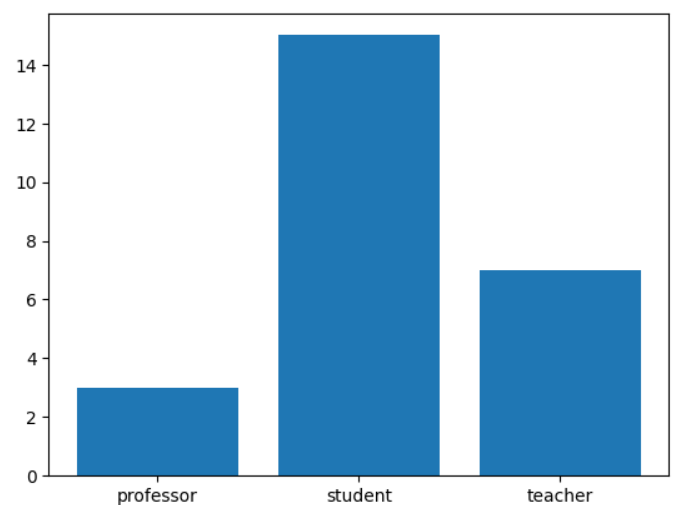
\includegraphics[scale=0.75]{img/103-1}

\subsection{Кругові діаграми.}

Кругові діаграми (Pie charts) призначені для представлення даних, а не для їх дослідження!

Люди не дуже добре оцінюють площу або кути (наприклад, важко визначити, чи один сегмент становить 23 $\%$, а інший — 27 $\%$). Стовпчасті діаграми набагато простіші, оскільки люди точніше порівнюють довжини.

Порівняти дві різні кругові діаграми (наприклад, два періоди часу) майже неможливо. Неможливо легко додати смуги похибки, опорні лінії або точні порівняння.

Якщо ж ви, з якоїсь причини, вирішили побудувати кругову діаграму (наприклад, щоб прпродемонструвати одемонструвтаи клієнту), ось приклад того, як це можна зробити:

\begin{lstlisting}
data = {"pie": 3,
        "pizza": 8,
        "apple": 12,
        "lavash": 11,
        "hat": 4}

plt.pie(data.values(), labels=data.keys(), autopct='%1.1f%%')
plt.axis('equal')
\end{lstlisting}

Результат:

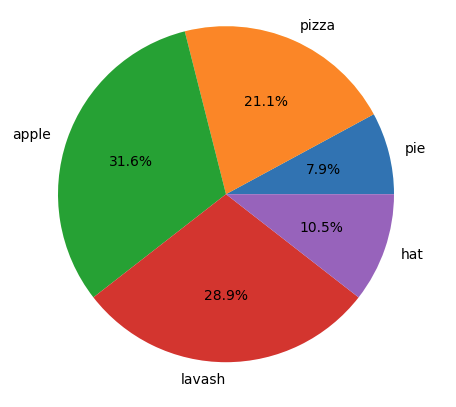
\includegraphics[scale=0.85]{img/103-2}



\subsection{Гістограми — числові дані}

Гістограма (Histogram) — це графік, який відображає розподіл числових даних, показуючи кількість спостережень у кожному інтервалі (біні).

\begin{lstlisting}
np.random.seed(0)
data = np.concatenate([30 + 4*np.random.randn(5000),
                       22 + 2*np.random.randn(7000),
                       12 + 3*np.random.randn(3000)])
plt.hist(data, bins=50)


# data = np.concatenate([10 + 5*np.random.randn(10000)])
# plt.hist(data, bins=50);
\end{lstlisting}

Результат:

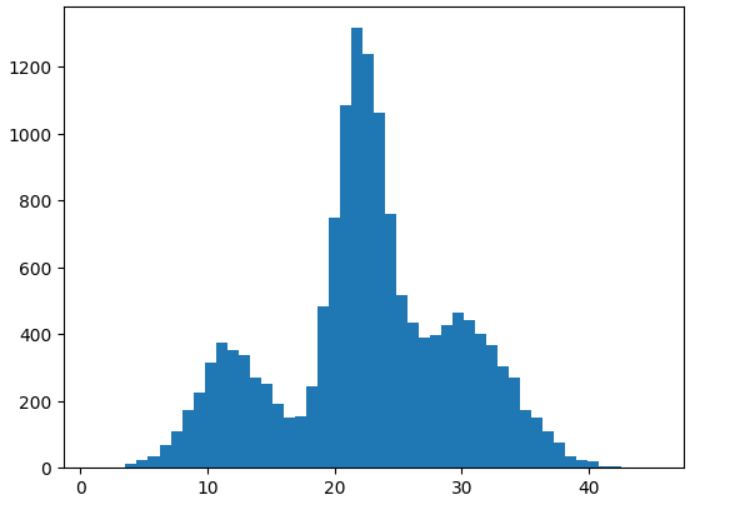
\includegraphics[scale=0.75]{img/103-3}

Гістограма показує розподіл числових даних, дозволяючи оцінити частоту появи значень у різних інтервалах. Бін (Bin) — це інтервал значень, у межах якого підраховується кількість спостережень. Занадто мала кількість інтервалів приховує деталі розподілу, тоді як занадто велика може зробити гістограму шумною та ускладнити її аналіз.



\section{2D дані}

\subsection{Точкові діаграми — числові x числові.}

Якщо обидва виміри даних є числовими, найприроднішим першим типом діаграми, який слід розглянути, є точкова діаграма (scatter plot): нанесення точок, які просто відповідають різним координатам даних. (Діаграма розсіювання)

\begin{lstlisting}
x = np.random.randn(1000)
y = 0.8*x**3 + x + 1.5*np.random.randn(1000)
plt.scatter(x,y,s=1)
\end{lstlisting}

Результат:

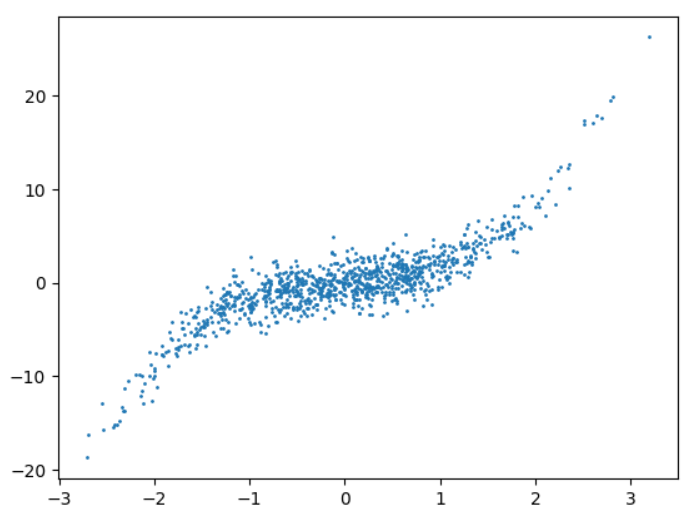
\includegraphics[scale=0.75]{img/103-4}


Однак існує також природний режим відмови, коли точок занадто багато, щоб їх можна було чітко розділити, і графік втрачає здатність показувати щільність даних. Наприклад, якщо у нас в 10 разів більше точок, графік вже не так чітко показує щільність у внутрішній частині "щільності".

У цьому випадку надлишку даних ми також можемо створити 2D гістограму даних (яка групує дані за обома вимірами) і вказати "висоту" кожного блоку за допомогою кольорової карти. Такі графіки можуть чіткіше вказувати щільність точок у регіонах, які в оригінальному графіку розсіювання мають суцільний колір. Ці 2D гістограми іноді також називають *тепловими картами* (heat maps), але ця назва часто конфліктує з подібними версіями, що використовуються для побудови 2D категоріальних даних, тому тут ми будемо використовувати термін *2D гістограма*.

\begin{lstlisting}
x = np.random.randn(10000)
y = 0.8*x**3 + x + 1.5*np.random.randn(10000)
#plt.scatter(x,y,s=10)

plt.hist2d(x,y,bins=100);
plt.colorbar();
plt.set_cmap('hot')
\end{lstlisting}

Результат:

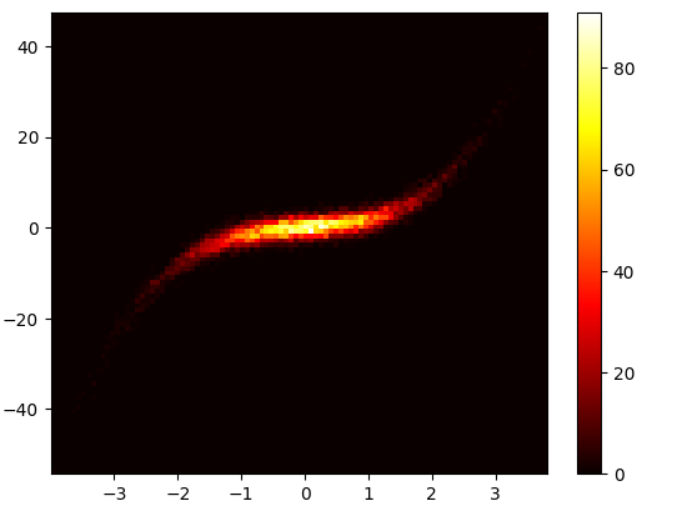
\includegraphics[scale=0.75]{img/103-5}


\subsection{Лінійна діаграма - числові x числові.}

Відомий всім зі школи і зрозумілий приклад візуалізації двовимірних числових даних, це лінійна діаграма (або графік, line plot). Це тип візуалізації, який відображає дані у вигляді точок, з'єднаних відрізками прямих.

\begin{lstlisting}
x = np.linspace(0,10,1000)
y = np.cumsum(0.01*np.random.randn(1000))
plt.plot(x,y)
\end{lstlisting}

Результат:

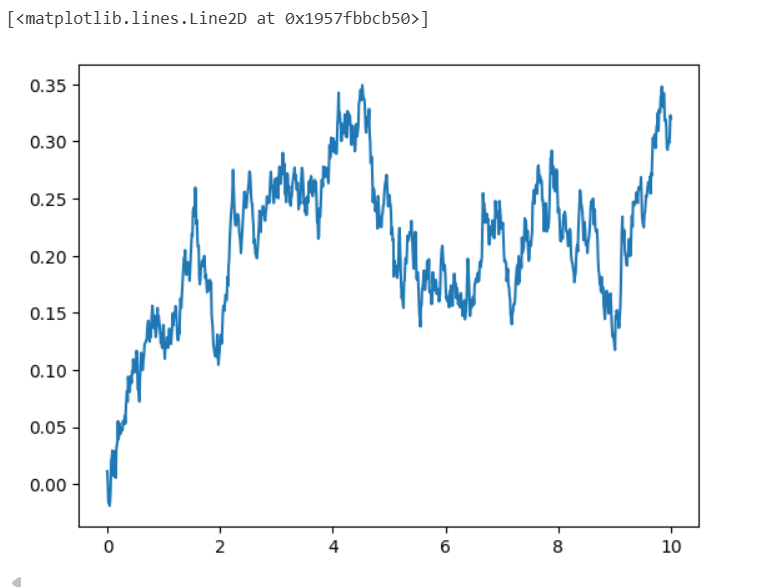
\includegraphics[scale=0.75]{img/103-6}




\subsection{Коробкова і скрипкові діаграми — категоріальні x числові}

Розглянемо простий приклад, де (тільки з вигаданими даними) ми будуємо графік учасників навчального процесу та їхній вік.

\begin{lstlisting}
import numpy as np
import matplotlib.pyplot as plt
import scipy.linalg as la

data= {"student": 22 + 1.4*np.random.randn(1000),
       "teacher": 37 + 2.5*np.random.randn(900),
       "professor": 65 + 5.5*np.random.randn(300)}
plt.scatter(np.concatenate([i*np.ones(len(x)) for i,x in enumerate(data.values())]),
            np.concatenate(list(data.values())))
plt.xticks(range(len(data)), data.keys());
\end{lstlisting}

Результат:

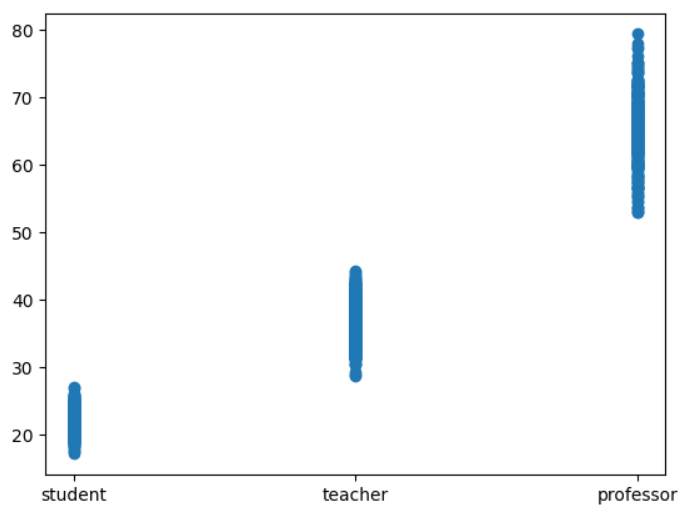
\includegraphics[scale=0.75]{img/103-7}


Очевидно, що, дивлячись тільки на цей графік, можна отримати дуже мало, оскільки в щільній лінії точок недостатньо інформації, щоб дійсно зрозуміти розподіл числової змінної для кожної точки. Поширеною стратегією тут є використання графіка коробкова, або коробка з вусами (box and whiskers), яка відображає медіану даних (як лінію в середині коробки), 25-й і 75-й процентилі даних (як нижня і верхня межі коробки), "вуса" встановлюються за допомогою ряду різних можливих угод (за замовчуванням Matplotlib використовує 1,5-кратний інтерквартильний розмах, відстань між 25-м і 75-м процентилем), а будь-які точки поза цим діапазоном ("випадкові значення", або "викиди") відображаються окремо.

\begin{lstlisting}
plt.boxplot(data.values())
plt.xticks(range(1,len(data)+1), data.keys())
\end{lstlisting}

Результат:

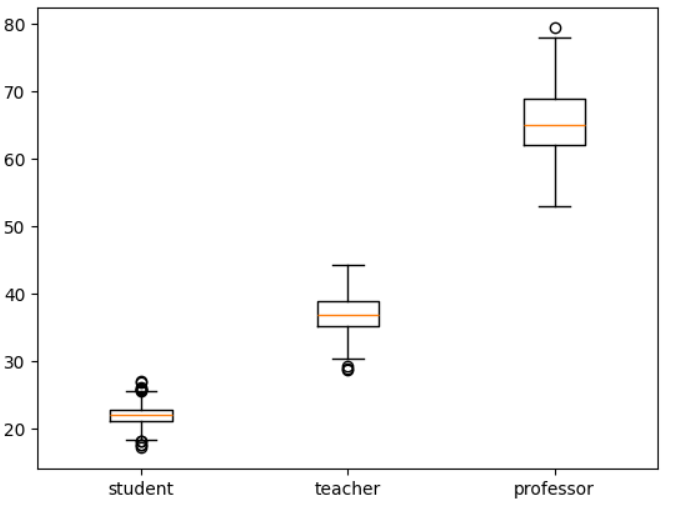
\includegraphics[scale=0.75]{img/103-8}


\ding{43} Звичайно, так само як середні значення та стандартні відхилення не описують повністю набір даних, статистика бокс-плат і вусів не відображає повністю розподіл даних. З цієї причини також часто використовуються скрипкові діаграми (violin plots), які створюють міні-гістограми.

\begin{lstlisting}
plt.violinplot(data.values())
plt.xticks(range(1,len(data)+1), data.keys())
\end{lstlisting}

Результат:

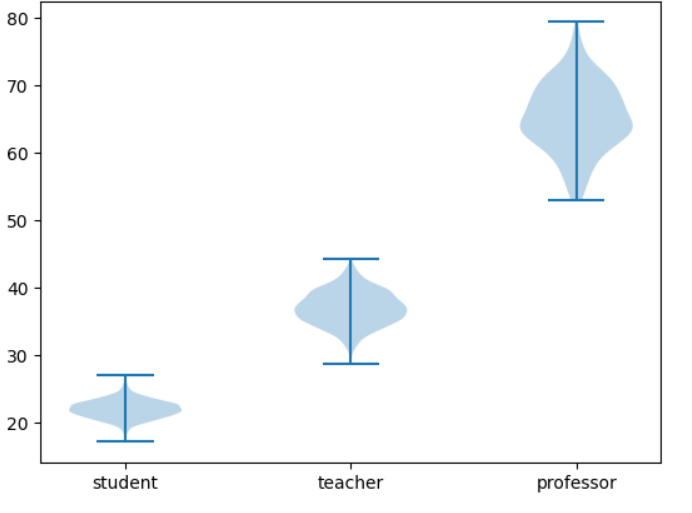
\includegraphics[scale=0.75]{img/103-9}


\subsection{Теплова карта та бульбашкові діаграми — категоріальні x категоріальні}

Теплова карта (Heatmap) — це спосіб візуалізації даних, у якому значення відображаються за допомогою кольорів, що дозволяє швидко оцінити їхню величину та закономірності. За допомогою теплових карт найчастіше візуалізують матриці кореляцій, статистичні таблиці, матриці відстаней, частоти спостережень та інші двовимірні числові дані. Теплова карта кореляцій використовується для наочного відображення сили та напряму кореляції між числовими ознаками, що допомагає виявити сильно пов'язані або незалежні змінні.

Коли обидва виміри наших 2D-даних є категоріальними, ми маємо ще менше інформації для використання. Знову ж таки, метою буде надання певної інформації про загальну кількість усіх можливих комбінацій між двома наборами даних. Наприклад, розглянемо вигаданий набір даних про учасників навчального процесу та їхній улюблений спосіб навчання.

\begin{lstlisting}
types = np.array([('student', 'offline'), ('student', 'remote'), 
                  ('teacher', 'offline'), ('teacher', 'remote'), 
                  ('professor', 'offline'), ('professor', 'remote')])
data = types[np.random.choice(range(6), 2000, p=[0.4, 0.1, 0.12, 0.18, 0.05, 0.15]),:]

# print(data[100:])

label_x, x = np.unique(data[:,0], return_inverse=True)
label_y, y = np.unique(data[:,1], return_inverse=True)
M, xt, yt, _ = plt.hist2d(x,y, bins=(len(label_x), len(label_y)))
plt.xticks((xt[:-1]+xt[1:])/2, label_x)
plt.yticks((yt[:-1]+yt[1:])/2, label_y)
plt.colorbar()
\end{lstlisting}

Результат:

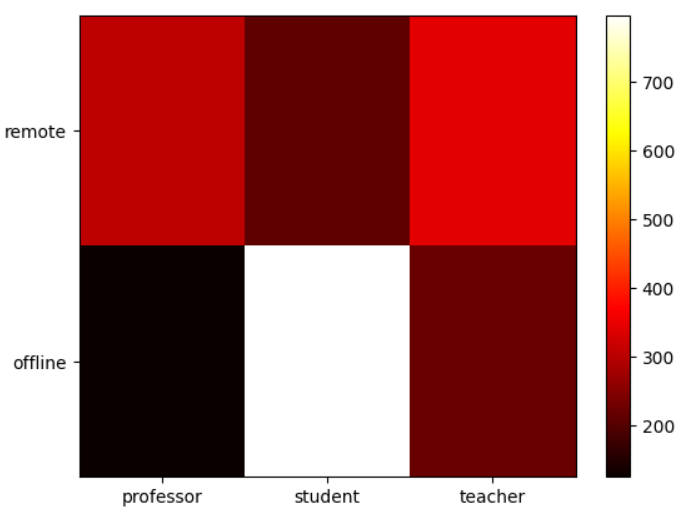
\includegraphics[scale=0.75]{img/103-10}

Хоча це може бути дещо корисним, діапазон кольорів, безперечно, не є дуже інформативним у деяких налаштуваннях, тому більш доречним може бути діаграма розсіювання з розмірами, пов'язаними з кожним типом даних (це також називається бульбашковою діаграмою).

\begin{lstlisting}
xy, cnts = np.unique((x,y), axis=1, return_counts=True)
plt.scatter(xy[0], xy[1], s=cnts*5)
plt.xticks(range(len(label_x)), label_x)
plt.yticks(range(len(label_y)), label_y)
\end{lstlisting}

Результат:

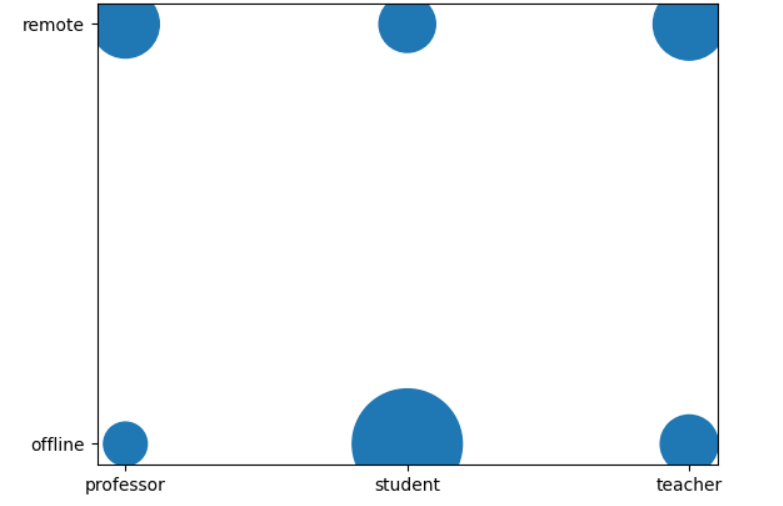
\includegraphics[scale=0.75]{img/103-11}

Бульбашкова діаграма (bubble plot) додатково використовує розмір маркерів для відображення ще однієї числової змінної. Розмір бульбашок може відображати величину показника, наприклад населення, прибуток, обсяг продажів або іншу числову характеристику.




\section{3D дані}


Як тільки ми виходимо за межі двох вимірів, ефективна візуалізація стає набагато складнішою.

3D точкові графіки (3D scatter plots), зображення точок в 3D, cлід уникати, якщо, звичайно, не можна взаємодіяти з 3D-графіком:

\begin{lstlisting}
x = np.random.randn(1000)
y = 0.4*x**3 + x + 1.7*np.random.randn(1000)
z = 0.5 + 0.1*(y-1)**2 + 0.4*np.random.randn(1000)

from mpl_toolkits.mplot3d import Axes3D
fig = plt.figure()
ax = fig.add_subplot(111, projection='3d')
ax.scatter(x,y,z)
\end{lstlisting}

Результат:

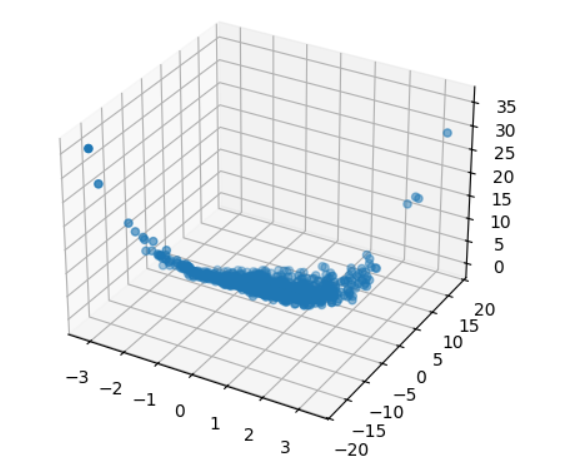
\includegraphics[scale=0.75]{img/103-12}


\subsection{Матриці розсіювання (точкові матриці).}

Універсальним засобом для візуалізації високорозмірних даних є матриця розсіювання (scatter matrices). 

По-суті, це сітка графіків, яка дозволяє візуально оцінити взаємозв'язок між усіма парами змінних у наборі даних. Тобто, для кожного набору двох із трьох аргументів, ми будуємо графік, враховуючи лише відповідні два агрументи, та ігноруючи третій. 

\ding{43} Щодо матриць розсіювання слід зазначити один важливий момент: не намагайтеся використовувати їх для представлення даних.

\begin{lstlisting}
import pandas as pd
df = pd.DataFrame([x,y,z]).transpose()
pd.plotting.scatter_matrix(df, hist_kwds={'bins':50})
\end{lstlisting}

Результат:

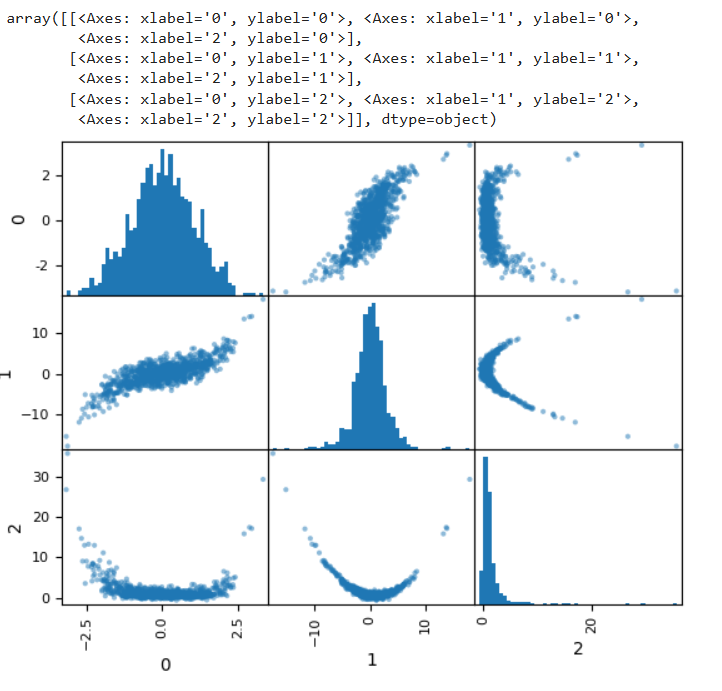
\includegraphics[scale=0.75]{img/103-13}


Матриця розсіювання використовується для одночасного аналізу взаємозв'язків між кількома числовими ознаками. За допомогою матриці розсіювання можна виявити кореляції, кластери, викиди (outliers) та можливі нелінійні залежності між ознаками.


\subsection{Бульбашкові діаграми.}

Бульбашкова діаграма (bubble plots) з попереднього розділу також може бути одним із засобів розуміння тривимірних даних. У цій діаграмі та її варіантах ми побудуємо двовимірну точкову діаграму, але додамо третій вимір за допомогою іншого атрибуту, наприклад розміру точок. Для наведених вище даних це буде виглядати наступним чином.

\begin{lstlisting}
plt.scatter(x,y,s=z*20)
\end{lstlisting}

Результат:

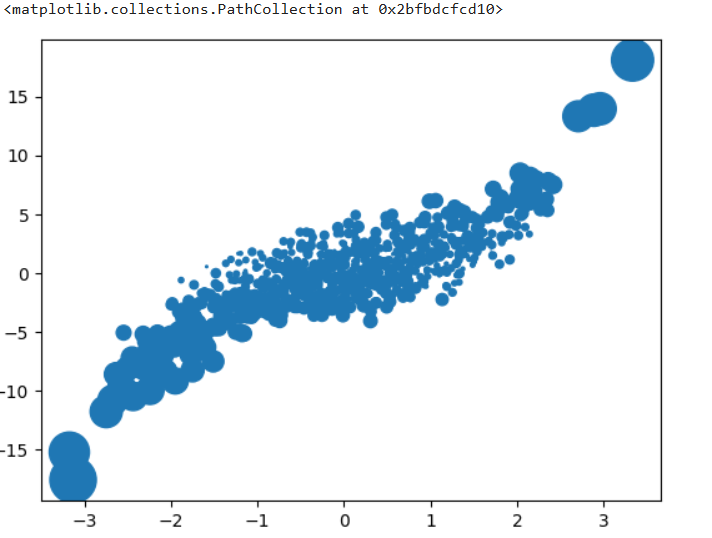
\includegraphics[scale=0.75]{img/103-14}


\begin{lstlisting}
plt.scatter(x,y,c=z)
\end{lstlisting}

Результат:

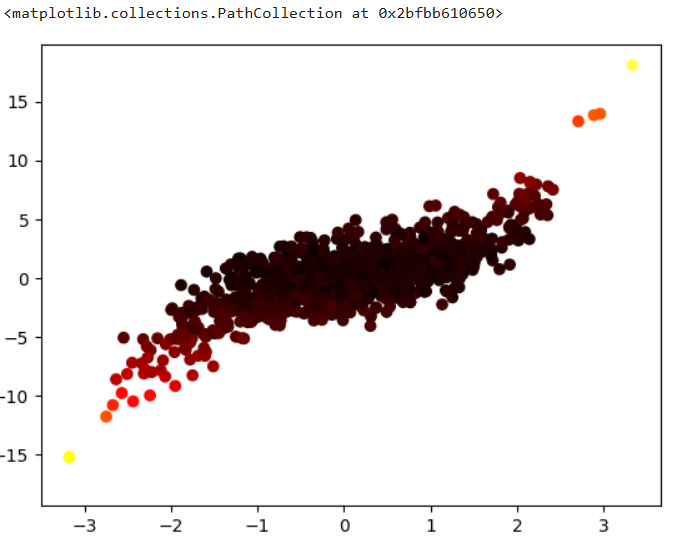
\includegraphics[scale=0.75]{img/103-15}


Тип діаграми обирають залежно від типу даних, кількості змінних, мети аналізу та закономірностей, які необхідно виявити. Правильно обрана візуалізація робить дані зрозумілішими, дозволяє швидко знаходити закономірності, виявляти аномалії та оцінювати взаємозв'язки між змінними.


\medskip

\ding{46} \textbf{Питання для самоконтролю.}


\begin{enumerate}
\item Що таке візуалізація даних і яке її значення в інтелектуальному аналізі даних?
\item Які основні цілі візуалізації даних?
\item Чому візуалізація є важливим етапом дослідницького аналізу даних (EDA)?
\item Які переваги має графічне представлення даних порівняно з табличним?
\item Які бібліотеки Python найчастіше використовуються для побудови графіків?
\item Які типи даних виділяють за шкалою вимірювання?
\item Що таке номінальні дані?
\item Наведіть приклади номінальних даних.
\item Що таке порядкові дані?
\item Наведіть приклади порядкових даних.
\item Що таке інтервальні дані?
\item Чим інтервальні дані відрізняються від даних співвідношення?
\item Що таке дані співвідношення (Ratio Data)?
\item Який тип діаграми найкраще підходить для номінальних даних?
\item Для яких типів даних доцільно використовувати гістограми?
\item Що таке стовпчаста діаграма (Bar Chart)?
\item Для яких задач використовується стовпчаста діаграма?
\item Чим стовпчаста діаграма відрізняється від гістограми?
\item Що таке кругова діаграма (Pie Chart)?
\item У яких випадках доцільно використовувати кругову діаграму?
\item Які недоліки має кругова діаграма?
\item Що таке гістограма?
\item Яку інформацію дозволяє отримати гістограма?
\item Що таке бін (Bin) у гістограмі?
\item Як вибір кількості інтервалів впливає на вигляд гістограми?
\item Що таке точкова діаграма (Scatter Plot)?
\item Для яких задач використовують точкові діаграми?
\item Як за допомогою точкової діаграми можна виявити кореляцію між змінними?
\item Що таке лінійна діаграма (Line Chart)?
\item Для яких типів даних найчастіше використовують лінійні діаграми?
\item Що таке коробкова діаграма (Box Plot)?
\item Які статистичні характеристики відображає коробкова діаграма?
\item Як за допомогою Box Plot можна виявити викиди?
\item Що таке скрипкова діаграма (Violin Plot)?
\item Чим скрипкова діаграма відрізняється від коробкової?
\item Що таке теплова карта (Heatmap)?
\item Які дані найчастіше візуалізують за допомогою теплової карти?
\item Для чого використовується теплова карта кореляцій?
\item Що таке бульбашкова діаграма (Bubble Chart)?
\item Чим бульбашкова діаграма відрізняється від звичайної точкової діаграми?
\item Яку інформацію може відображати розмір бульбашок?
\item Що таке матриця розсіювання (Scatter Matrix)?
\item Для чого використовується матриця розсіювання під час аналізу даних?
\item Які закономірності можна виявити за допомогою матриці розсіювання?
\item Що таке тривимірна (3D) візуалізація даних?
\item Які типи 3D-графіків підтримуються сучасними бібліотеками Python?
\item Які переваги має використання 3D-візуалізації?
\item Які недоліки та обмеження має 3D-візуалізація?
\item За якими критеріями слід обирати тип діаграми для конкретного набору даних?
\item Яким чином правильний вибір способу візуалізації допомагає виявляти закономірності, аномалії та взаємозв'язки у даних?
\end{enumerate}